\documentclass[twocolumn]{aastex62}
\bibliographystyle{aasjournal}

%\bibliographystyle{apj}
\usepackage{graphicx}
\usepackage[suffix=]{epstopdf}
\usepackage{natbib}
\usepackage{amsmath}
\usepackage{xspace}


%    Make Scientific Notation
\providecommand{\e}[1]{\ensuremath{\times 10^{#1}}}

% make the word Kepler italicized
\newcommand{\Kepler}{\textsl{Kepler}\xspace}


\begin{document}
%%%%%%%%%%%%%%%%%%%%%%
\title{SETI in the Spatial-Temporal Survey Domain}

\shorttitle{Survey SETI}
\shortauthors{Davenport}


\author{James. R. A. Davenport}
\affiliation{Department of Astronomy, University of Washington, Seattle, WA 98195, USA}
\altaffiliation{DIRAC Fellow}


%%%%%%%%%%%%%%%%%%%%%%%%%%%%%%
\begin{abstract}
Traditional searches for extraterrestrial intelligence (SETI) or ``technosignatures'' focus on dedicated observations of single stars or regions in the sky to detect excess or transient emission from intelligent sources. The latest generation of synoptic time domain surveys  enable an entirely new approach: spatial--temporal SETI, where technosignatures may be discovered from spatially resolved sources or multiple stars over time. 
Current optical time domain surveys such as ZTF and the Evryscope can probe 10--100 times more of the ``Cosmic Haystack'' parameter space volume than many radio SETI investigations. Small-aperture, high cadence surveys like Evryscope can be comparable in their Cosmic Haystack volume completeness to deeper surveys including LSST. Investigations with these surveys can also be conducted at a fraction of the cost, since they require analysis of data already being gathered. 
However, SETI methodology has not widely utilized such surveys, and the literature is in need of new search algorithms that can incorporate signals from both the spatial and temporal domains.
Here I describe the broad potential for modern wide-field time domain optical surveys to revolutionize our search for technosignatures, and illustrate some new example SETI approaches that utilize the spatial-temporal domain
\end{abstract}

%Here I propose one such SETI approach, which utilizes exoplanet-like transit signals coordinated around multiple stars to indicate the presence of an interstellar civilization. In this scenario, artificial occulting objects would act as beacons, being placed in orbit around stars surrounding the central home star system. The orbital period of each artificial satellite would be proportional to the distance from the beacon star to the home star system. If the orbital period versus beacon distance relationship was known, the exact location of the home system could be determined via triangulation (or trilateration) from a subset of the transiting beacons seen by an observer. Current and future exoplanet surveys would be able to detect such spatially coordinated transits around nearby low-mass stars. While contrived, this example highlights the need for SETI researchers to consider the spatial-temporal domain.


%\keywords{stars: activity --- stars: low-mass --- planets and satellites: detection}


%%%%%%%%%%%%%%%%%%%%%%%%%%%%%%
\section{Introduction}

Despite more than half a century of activity, the Search for Extra-Terrestrial Intelligence (SETI) is a field of study very much in its infancy. 
\citet{wright2018c} note the volume of parameter space for SETI (or the search for a needle amongst the ``cosmic haystack'') at radio wavelengths has been barely explored, and that many obvious signals may indeed be awaiting our discovery. 
The lack of SETI activity by the astronomical community can be partially understood as due to funding limitations in recent decades, as well as social pressures against studying SETI experienced by professional astronomers and organizations \citep{wright2018b}. 


Traditional SETI work also requires time-consuming observations, often through dedicated monitoring of nearby stars by radio telescopes. Such observing campaigns are expensive and difficult to obtain given the competitive nature of telescope allocation. Recent progress for systematic ``technosignature'' searchs has been made by Breakthrough Listen \citep{worden2017,isaacson2017}, primarily at radio wavelengths \citep[e.g.][]{price2018}. 


The SETI conundrum has always been not only ``{\it What should we look for?}'', but  also {\it ``When, where, and how to look?}''. 
While \citet{wright2018c} suggest the completeness of our search of the ``cosmic haystack'' at radio wavelengths is akin to the ratio of a swimming pool compared to the Earth's ocean's ($\sim$10$^{-20}$), SETI at optical wavelengths is surely many orders of magnitude less complete. However, new wide-field time domain surveys will enable us to greatly expand our search in two key dimensions of parameter space: 1) collectively observing nearly the entire night sky, and 2) providing time resolved monitoring over many years. 


Surveys like the currently running Zwicky Transient Facility \citep[ZTF][]{bellm2014} and the upcoming Large Synoptic Survey Telescope \citep[LSST][]{lsst} will be transformative in enabling both reproducible and cost-efficient SETI. By developing search strategies that utilize public survey databases and real-time ``alert streams'', both of which are being developed to facilitate a wide range of science goals from these facilities, optical survey SETI can be conducted automatically. As new search algorithms are developed, these databases can be quickly re-analyzed, providing a much-needed level of reproducibility and transparency that will help reduce the ``giggle factor'' stigma for SETI \citep{wright2018b}.


In this paper I explore the potential for wide-field time domain surveys in conducting a new generation of technosignature searches, starting with an overview of the motivation for doing SETI with optical surveys in \S\ref{sec:method}.
In \S\ref{sec:strategy} I describe the general principles behind technosignature searches in time domain surveys, including spatial over-densities of light curve signals and coordinated signals between multiple sources, for example.
In \S\ref{sec:haystack} I introduce several relevant surveys, and use the ``Cosmic Haystack'' search volume metric developed by \citet{wright2018c} to quantitatively compare these surveys to current radio SETI approaches. 
The data-driven spatial-temporal domain explored by these surveys necessitates new SETI approaches be developed, and in \S\ref{sec:transit} I outline an example signal where transiting planets around many stars could act as a spatially distributed beacon network.
Finally in \S\ref{sec:discussion} I discuss ideas for other search approaches, and the advantages in cost and reproducibility of conducting SETI with current and upcoming optical time domain surveys.

%\bf THE POINT: } in this new spatial-temporal domain, we should be looking for things that happen in space, such as over densities of events, or coordination of events like transits.




%{\bf THIS PAPER NEEDS TO BE RETHOUGHT, IN LIGHT OF MORE SPECIFIC PAPER IDEA:}{\it SETI with ZTF}
%
%In the search for extraterrestrial intelligence (SETI), most approaches focus on direct detection of photons originating from transmission or waste energy. These searches occur over a range of wavelength regimes, and assume an extraterrestrial civilization will produce sufficient radiation to be detected apart from their parent star. While this may be feasible at radio wavelengths where Sun-like stars have lower emission, it is much more difficult to outshine the star in the optical regime where many present-day time domain surveys operate. 
%
%
%Blocking a significant fraction of light from a star may instead be much easier than outshining it \cite{arnold2005}. This has led to recent searches for transit-like signatures that may have artificial origins. For example, PAPER demonstrated the observable impact of transits by non-spherical objects \cite{arnold2005a}.
%on the impact of artificial structures on transits. also this work on that:
%\cite{wright2016}.
%recent data from \Kepler \citep{borucki2010}, has found weird transit-like signals
%\cite{boyajian2015}, 
%which some have considered as SETI candidates. However, follow-up observations have yet to yield any confirming signatures, and instead this looks like a YSO w/ comets maybe \citep{lisse2015}.
%
%
%Previous work has suggested looking for SETI signals from interstellar ``beacons''
%\cite{benford2008}
%However, most such work has been focused on using lasers or other means to out-shine a parent star, often observed using spectroscopy \cite{reines2002}. This is a very expensive way to stand out, and a slow way to find it, and so far has no success in discovering ET laser emission \cite{tellis2015}
%\cite{arnold2005} note that objects could be placed at interesting spacing along the orbit to encode a pattern or simple message, demonstrating an intelligent origin. However, very little information can be effectively transmitted using eclipses, even with extreme precision in the recovery.
%\cite{forgan2017} show a galactic-scale communications network of using transits, but note links in the network are only stable for order $10^5$ years as galactic orbital dynamics move things around



%optical seti
%\citep{holder2005} optical pulse SETI 
%
%a review of Schelling points from \citet{wright2017}
%lighthouses \citep{zuluaga2015}
%active and passive SETI in coordination (both temporal and spatial) with galactic events like supernovae 
%\citep{lemarchand1994}
%coordinated times/places, also known as Schelling or Focal points \citep{schelling1960}, are the key to finding people in unknown time/space.
%planets in Earth's transit zone \cite{heller2016} - maybe transits would be aligned for our viewing benefit?
%


% include mantras of "worth doing", "do it almost for free", "reproducible", "portable, do it everywhere", and "outliers are nature papers"

%%%%%%%%%%%%%%%%
\section{Why Optical Survey SETI?}
\label{sec:method}

% The first SETI challenges: WHEN, WHERE, WHAT to search
Wide-field imaging surveys, and their associated infrastructure, are an ideal data source for carrying out technosignature searches that augment efforts in other wavelengths or with different observing strategies. By covering large portions of the night sky with repeated imaging, and with surveys that span years to decades in duration, we can substantially reduce the challenge of deciding {\it when} and {\it where} to look. Increasingly, multiple surveys obtain imaging that overlaps in both time and sky coverage, but with complimentary properties (e.g. imaging depth, cadence, wavelength coverage), which allows for rapid vetting and characterization of rare or low signal-to-noise events.. This also results in survey data providing some ``ground truth'' about the nature of most known objects in our Galaxy (e.g. their positions, temperatures, etc), and allows us to eliminate uncertainty on {\it what} objects we're studying for SETI.

% next: HOW to search (can compare approaches, and make them reproducible)
Optical surveys are also an excellent platform for exploring {\it how} to conduct technosignature searches. The large archives of data produced from these surveys become valuable legacies that enable science long after data acquisition has concluded. Searches for new phenomena in time-domain astronomy can be carried out both in the future with new observations and in the past by re-analyzing survey archives. 
Using survey archives for SETI as opposed to targeted observations allows us to compare the results of competing algorithms or strategies, and enables reproducible science. Search algorithms are also portable, and ideally can be used to carry out SETI on any appropriately structured large survey.
As future survey data is gathered, new classes of technosignature signals may be detectable that rely on decades worth of data. 
Since any candidate technosignature detection will (or should) be the subject of great scrutiny, making the data and algorithms open and reproducible will be critical for comparison and independent validation. 


% DO IT FOR "FREE"
Large surveys, particularly ground-based efforts like LSST, are a highly prioritized component of the current and future development landscape in astronomy \citep{astro2010}. As such, great efforts are being made to develop survey tools and technologies to enable science from these missions, such as new database technologies \citep{juric2012}. These developments are especially needed to utilize the new forms of data being made available, including real-time data analysis \citep[e.g.][]{schwamb2019} and broadcasting real-time alerts for events \citep{patterson2019}.
The infrastructure needed to conduct technosignature searches with these large optical surveys is therefore already being developed. As with many areas of astrophysics in the ``survey era'', the biggest restriction to SETI with large surveys is therefore the availability of supported researchers mine the data.




%%%%%%%%%%%%%%%%%%%%%%%%%%%%%%
\section{Potential Strategies}
\label{sec:strategy}

SETI with large surveys falls into two basic approaches: 1) classify every object or phenomena in the data, and any remaining outliers are technosignature candidates, or 2) search for specific ``impossible'' or unusual types of signals in the data, which I advocate for in this work. While the latter strategy does not guarantee a complete search for all SETI signals in the data, it is technically feasible for almost any time domain survey. 

Several types of signals have been suggested that may be viable for use with optical surveys. For example, \citet{villarroel2016} searched two wide field, single-epoch optical surveys for objects ``disappearing''  over decades timescales. \citet{lacki2019} outline a method to search for specular reflections of interplanetary objects, particularly in wide field surveys. \citet{arnold2005} describe the the observable signature of transits from artificial objects, which could be searched for with exoplanet transit surveys. \citet{kipping2016} find that exoplanet transits could be hidden or ``cloaked'' to an observer by using directed laser emission.

Here I describe a few general classes of technosignature signals that may be well suited to developing new detection algorithms for spatial-temporal surveys:

\begin{enumerate}
\item {\bf Unusual variability profiles or statistical distributions of fluxes }-- either on short timescales such as Boyajian's Star \citep{boyajian2015}, or long timescales such as disappearing stars \citep{villarroel2016} or occasionally missing transits \citep{kipping2016}
%
\item {\bf Spatial correlations of events or phenomena }-- e.g. coordination of transiting systems, or rebroadcasting events such as novae along the ``SETI ellipse'' \citep{makovetskii1977,lemarchand1994,tarter2001,shostak2004}
%
\item {\bf Spatial over-density or distribution} -- e.g. an over-density of a given phenomena, such as within the Earth Transit Zone \citep{heller2016}
%
\item {\bf Unnatural patterns} -- particularly patterns of otherwise normal astrophysical variability, such as broadcasting a prime or fibonacci sequence of transits \citep{wright2016}.
%
\end{enumerate}




%%%%%%%%%%%%%%%%
\section{Comparing Optical Surveys\\ to Radio Searches}
\label{sec:haystack}

\citet{wright2018c} have provided a framework to quantify the volume of observable parameter space covered by various SETI projects -- dubbed the ``Cosmic Haystack''. The properties for several major radio SETI projects yield a Haystack volume coverage of $10^{-20}$ to $10^{-18}$, or as \citet{wright2018c} illustrate, akin to a drinking glass of water compared to the volume of Earth's oceans. While this tool was developed with radio surveys in mind, it is broadly applicable to surveys at other wavelengths that are not explicitly designed for SETI \citep[e.g. see][]{forgan2019}.


While the potential for optical time domain surveys to advance technosignature searches has been qualitatively laid out in \S\ref{sec:method}, it is useful to quantitatively compare their capability to traditional searches in the radio. 
For typical optical surveys using broadband photometry \citep{djorgovski2013}, the key parameters that determine the Cosmic Haystack volume coverage are the sky coverage ($\Omega$ in sq deg), total integration time per target ($T$ in sec), and survey sensitivity or per-epoch depth ($S$ in Jy).
%we need to be looking at big optical surveys, since they provide such amazing sky/time coverage


Evryscope \citep{law2015} is amazing

starting to probe fainter sources becomes a trade off for area and time coverage.
Zwicky Transient Facility \citep{bellm2014}
for example surveys the sky every couple nights, but with only a single visit per source per night.


%space-based platforms designed for exoplanet searches provide very high quality light curves over months to years timescales. The \Kepler and K2 missions \citep{borucki2010,howell2014} produced 30-minute cadence light curves for $\sim$500,000 stars, with baselines ranging from $\sim$3 months up to 4 years. 
and TESS \citep{tess}, as well as Gaia \citep{gaia} provide incredible precision light curves for millions of stars.






\begin{figure}[]
\centering
\includegraphics[width=3.5in]{../figures/optical_haystack}
\caption{
comparison of the 8D ``Cosmic Haystack'' volume defined by \citet{wright2018c} using five optical surveys with varying designs. 
}
\label{fig:hay}
\end{figure}



%%%%%%%%%%%%%%%%%%%%%%%%%%%%%%
\section{Example: Spatial-Temporal\\ Transit Beacons}
%\section{Example 1: Coordinated Transits as ET Beacons}
\label{sec:transit}


\subsection{Coordinated Transit Networks}
imagine a Type N civilization with the ability to both travel to nearby star systems, and to build large enough structures in orbit around other stars to produce a visible transit in our data.

give the detailed example i have thought up.

becons placed at distances


\begin{figure*}[]
\centering
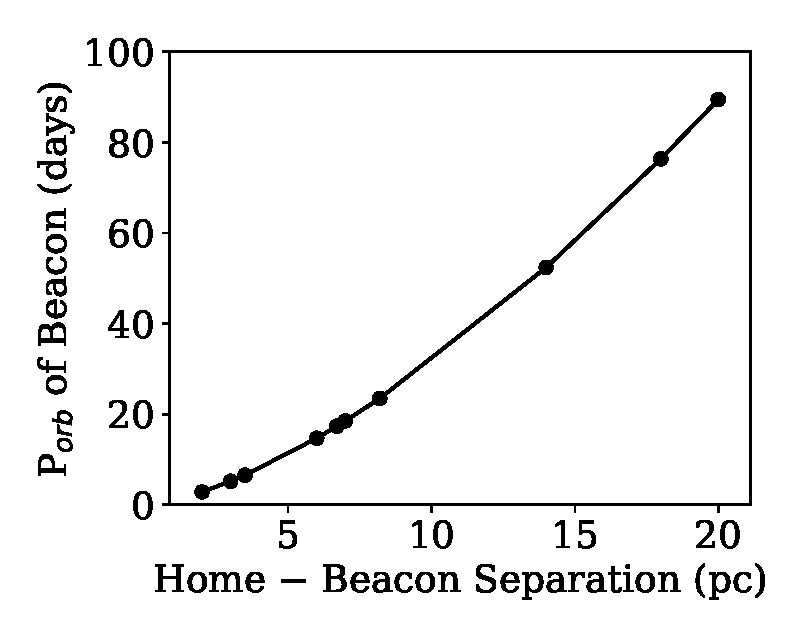
\includegraphics[width=2.75in]{../figures/dist_per.pdf}
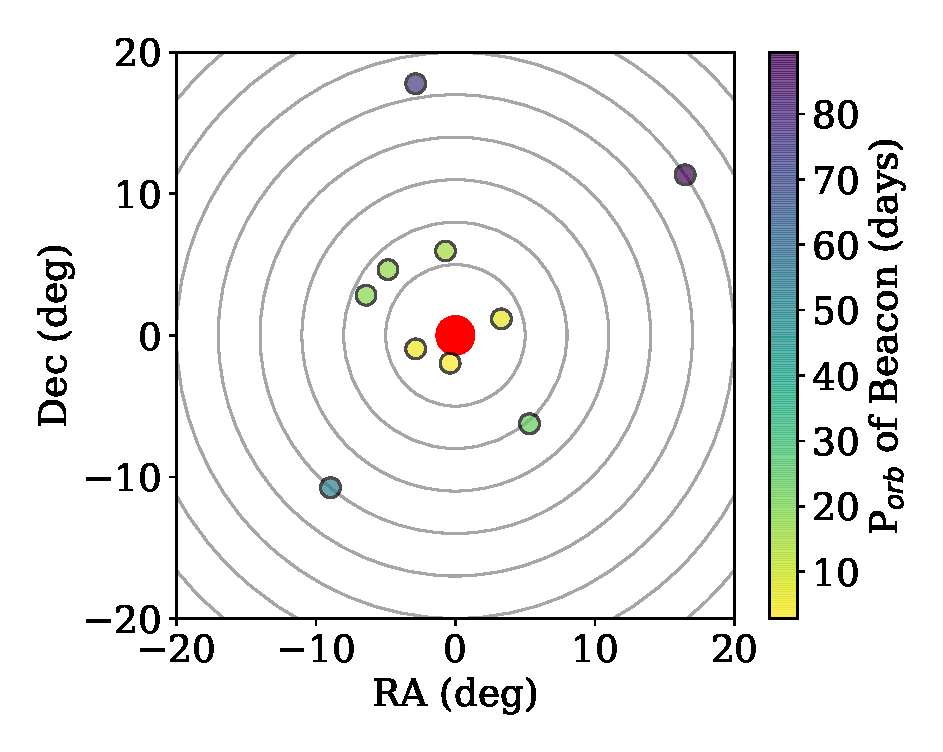
\includegraphics[width=2.75in]{../figures/sky_per.pdf}
\caption{schematic figure of the signal to detect in 2 dimensions. ra,dec in arbitrary units. red circle in middle is the home system}
\label{fig:2d}
\end{figure*}


for clarity, this is what the ideal signal might look like on the sky


%%%

this type of beacon network is advantageous because it points directly back towards their home. only a few systems actually need to be transiting from any given line of sight.

NOW THE FULL SIMULATION...
- computation to do: if had 100 beacons, each placed at random orbital alignment, in 3d sphere around home system.
- assume G stars, 
- odds of observing transit of a fixed sized object versus orbital distance... goes down. need that plot to figure out probability. 
- assume ET places beacons with uniform RADIAL density in 3d space out to some maximum distance (even \# of systems as function of radial distance) in bins of 10pc out to 100 pc (i.e. 10 beacons in each 10pc bin)
- orbital period is exact for each system, no bins of period
- do Monte Carlo sim with these parameters to figure out how many transiting systems we'd observe 

---- make the plot for one MC realization of RA,Dec.... open circles for systems with no observed transits, colored for transits

\begin{figure}[]
\centering
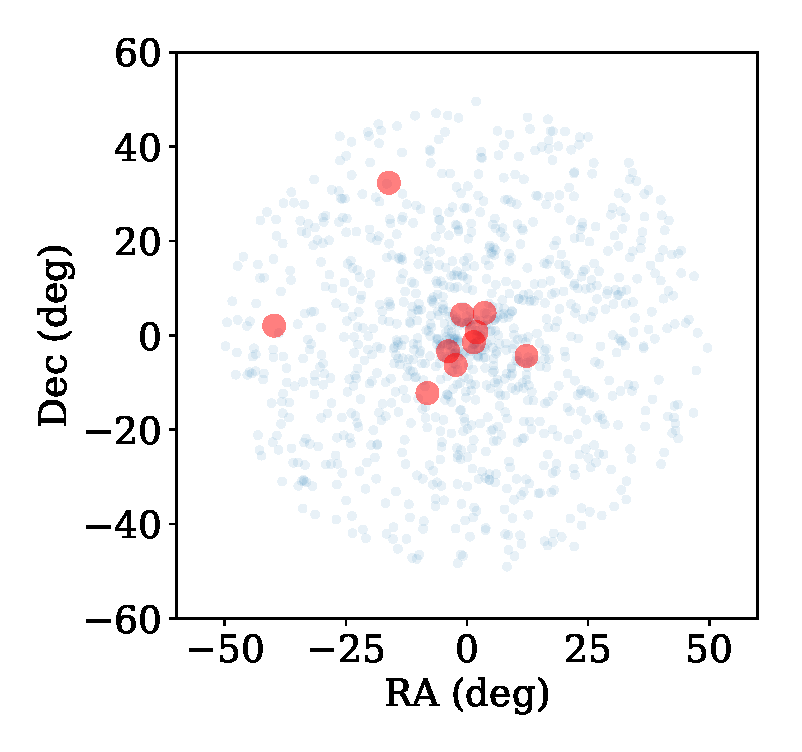
\includegraphics[width=3in]{../figures/3d_model.pdf}
\caption{the model in 3 dimensions projected into the sky plane. 1000 simulated systems that span the galactic distance of 5-50 pc (blue) with 10 recovered transits highlighted (red). these would be hot Jupiters at the short P end.}
\label{fig:3d}
\end{figure}

\begin{figure}[]
\centering
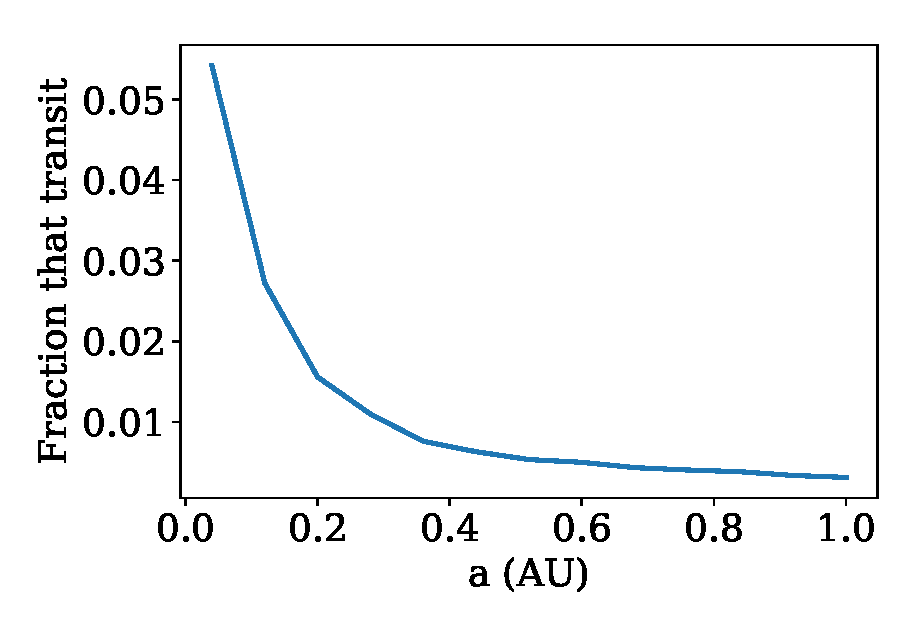
\includegraphics[width=3in]{../figures/recov_fraction.pdf}
\caption{fraction of hot Jupiter-like systems recovered in 1000 realizations of our 1000-star simulation. This curve is dependent on the ratio of the occulter-to-star size, and the orbital period range sampled.
The average from our model is $10\pm 3$ systems recovered for these parameters.}
\label{fig:recov}
\end{figure}


IDEA:
could improve the efficiency of these beacons if we consider a bit of galactic structure, aligning the median orbital inclinations of the beacon systems with the Galactic plane, and only allowing a smaller range of possible inclinations. How much more efficient would it be if we forced $i<10^\circ$, instead of $i<90^\circ$?

for a million system model w/ 90deg max, 0.46\% total detection efficiency. 
by constraining the inclination to 10deg max, get 4.3\% detection efficiency of planets. 30deg max gets 1.4\%


PROBLEM:
as \citet{forgan2017} note, an interstellar communications based on transits may only be stable for $\sim$10,000 years due to evolution of planetary orbits and relative motion between stars within the Milky Way. The beacon systems centered around the host system would have to be traveling as a moving group to maintain their respective trilateration signals, or have the transiting bodies actively over time. In other words, as the beacon systems moved relative to the ET host star due to differing Galactic orbits, the semi-major axis of the transiting bodies would have to be adjusted to compensate.



%%%%%%%
\subsection{Searching for Correlated Transits in Kepler}
we compute the 2-point correlation between all transits in the Kepler sample in 2D space (radius)

we find there is no correlation. Thats OK, but at least we searched

\citet{coughlin2014} find some correlations that are apparently removed in KOI catalog creation... due to contamination by RRlyr or other thing?
See also TCE histogram in \citet{twicken2016}



\begin{figure}[]
\centering
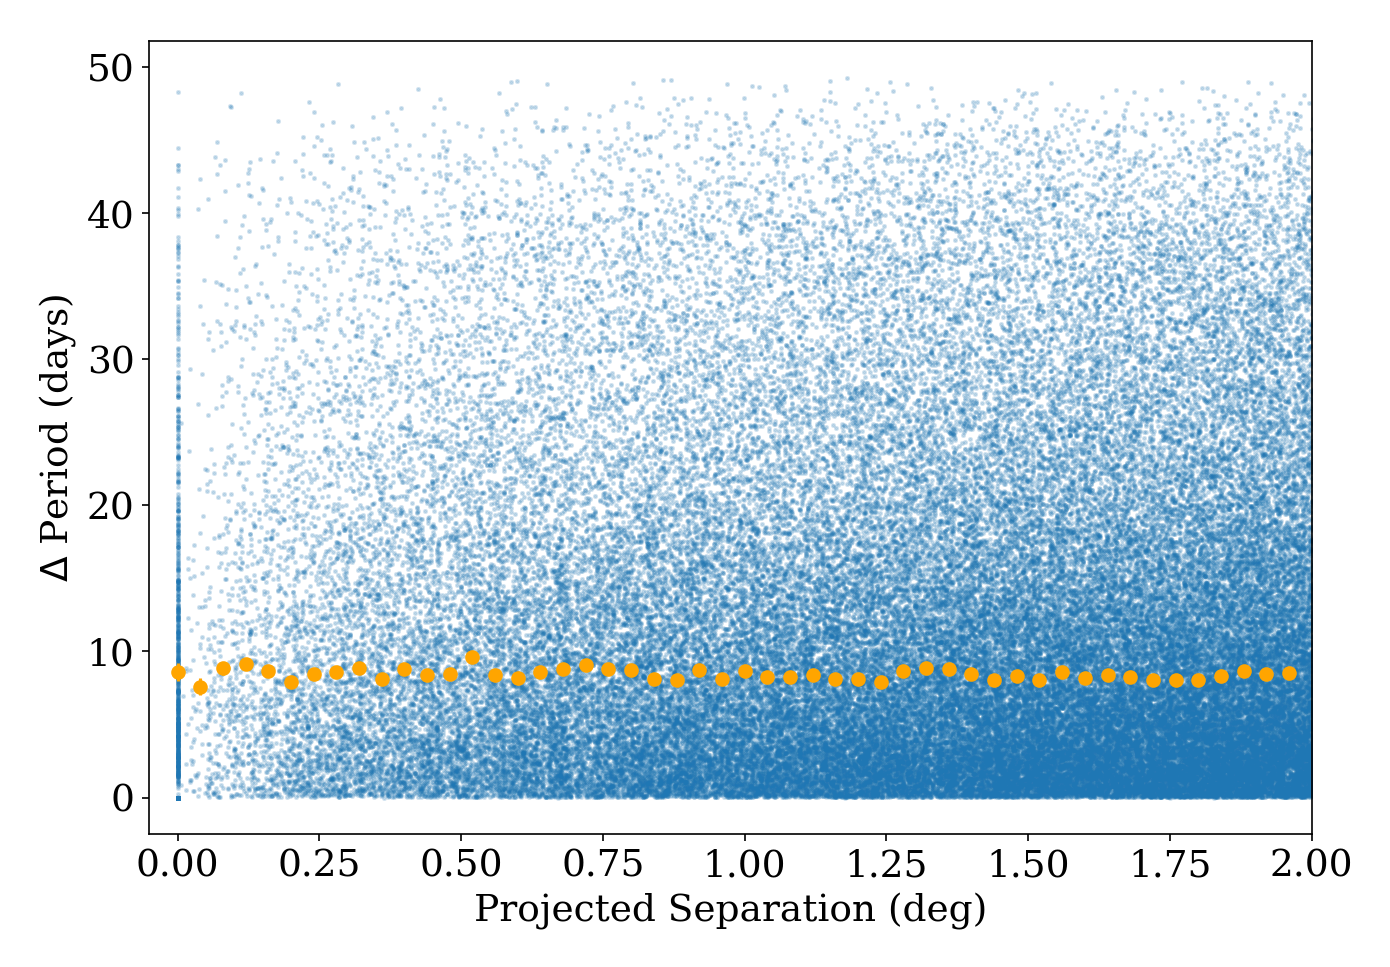
\includegraphics[width=3in]{../figures/delta_per.png}
\caption{searching for correlation between transit periods and projected separations between all exoplanet systems out to 2deg in the Kepler data. 
median period differences are computed for bins of separation distance (orange points).
there is no trend in these medians, indicating a distribution of orbital periods that are random on large scales.}
\label{fig:2dcor}
\end{figure}



%\begin{figure}[]
%\centering
%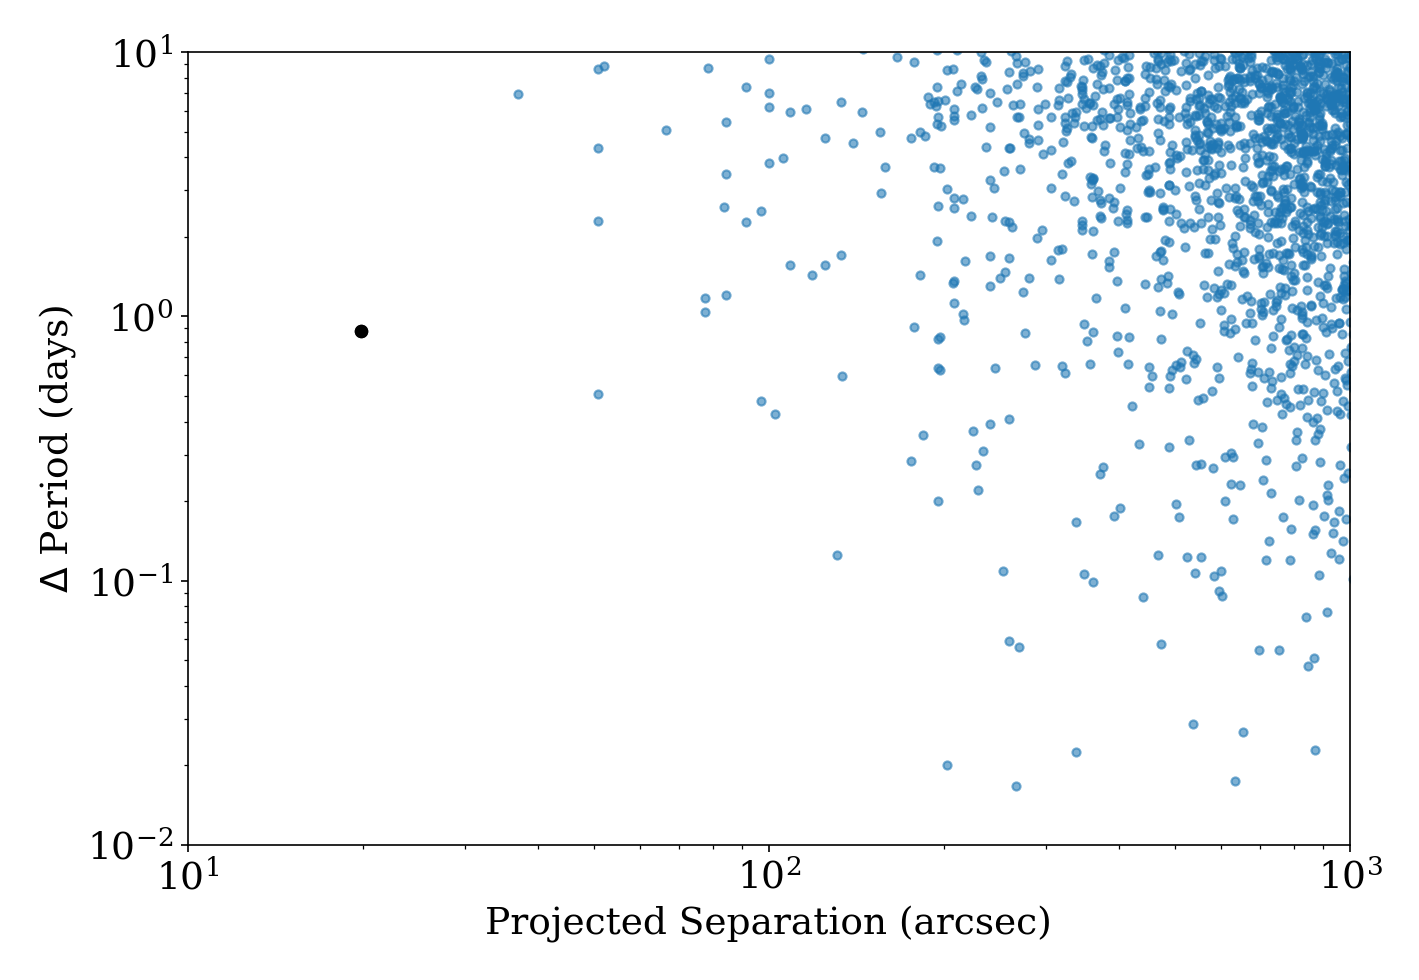
\includegraphics[width=3in]{../figures/delta_per2.png}
%\caption{correlation between transit periods and projected separations, as in Figure \ref{fig:2dcor}, but emphasizing the smallest separations in both axes. One outlier was identified in the similarity of Kepler 1292b and Kepler 1235b (black circle). However, these two systems are more than 600 pc separated in distance.}
%\label{fig:2dcor2}
%\end{figure}




%%%%%%%%%%%%%%%%%%%%%%%%%%%%%%
\section{Discussion}
\label{sec:discussion}
%
%to get accurate census you need a complete time domain survey at some transit depth sensitivity out to some orbital period. going off our simulation, TESS might work for very short period planets
%
%TESS would be great for this in terms of spatial-temporal coverage. 
%
%LSST very good for finding SETI signals of this geometric style, but not ideal for events requiring such dedicating monitoring
%
%this kind of distributed network could be very efficient at broadcasting the presence of a civilization. dust clouds could create sufficient "transit" signals, while not affecting orbital dynamics


so far we have focused on the need for developing SETI approaches that utilize the new spatial-temporal domain. The data streams from these surveys also enable many other search strategies that could be implemented. these might include:
VASCO-type events, stars appearing or disappearing. \citep{villarroel2016}
	- Esp. stars appearing that do not have a Gaia DR2 detection, for example.
	- need to account for novae, etc...
	- stars disappearing will be very interesting

coordination/synchronization \citep{makovetskii1977,shostak2004}
        - especially the SETI ellipsoid, a'la SN1987A \citep{lemarchand1994}
        - could use galactic novae to provide time/place
        - %https://asd.gsfc.nasa.gov/Koji.Mukai/novae/novae.html (new Novae)
        - %http://www.cbat.eps.harvard.edu/nova_list.html historic Novae (till 2010)

unnaturals patterns of otherwise normal events
	- look for e.g. flares or novae that recur w/ prime or fibonacci sequences
	- see forthcoming paper




Surveys like ZTF (and soon LSST) publish real-time alerts of variability from sources. These alert streams could be monitored in real-time for signals as well:
alerts from the stars within the ``restricted Earth Transit Zone'' \citep{heller2016}
	- anytime we can see them w/ ZTF
	- especially at our opposition (i.e. when we transit)
	- with Gaia we can track stars that are leaving the ETZ as well, but might 
	have seen us transit previously (or by the time the signal reaches us)

alerts from known exoplanet host systems, especially coinciding with any known transit conjunction (mid-transit), 
	- allow some tolerance window to account for TTVs



The cost of deploying such SETI is remarkably low, since they can ``piggyback'' on databases and search tools being developed for the primary science drivers of each survey (e.g. transients for ZTF).


%Lastly, we should resist the impulse to try and develop every possible search algorithm to mine this wealth of data for technosignatures. Instead, immediate progress can be made in SETI by deploying robust algorithms to search for specific signals


%%%%%%%%%%%%%%%%%
\acknowledgments

The author thanks Nicholas M. Law and Jason T. Wright for their helpful ongoing conversations in developing this idea, and Andrew P. V. Siemion and the Berkeley SETI Research Center team for hosting me for an enlightening and motivating visit.

JRAD acknowledges support from the DIRAC Institute in the Department of Astronomy at the University of Washington. The DIRAC Institute is supported through generous gifts from the Charles and Lisa Simonyi Fund for Arts and Sciences, and the Washington Research Foundation.

\bibliography{/Users/james/Dropbox/references}

\end{document}